\startappendix{Kinematic Distributions (N-1) in Signal Regions}
\label{chapter:appendix_SR_N_1}

Figures \ref{fig:Nminus1mergedSR_app} and \ref{fig:Nminus1resolvedSR_app} show N-1 plots with the finalized selections for the variables listed in Table \ref{tab:opt_vars} that used to define the analysis regions that are not shown in Figures \ref{fig:Nminus1mergedSR} and \ref{fig:Nminus1resolvedSR_app}, respectively, in Section \ref{sec:sr_selection}. The placements of cuts is also shown using red arrows.

\begin{figure}[htbp]
  \centering
    \begin{subfigure}[t]{0.48\textwidth}
    \centering
     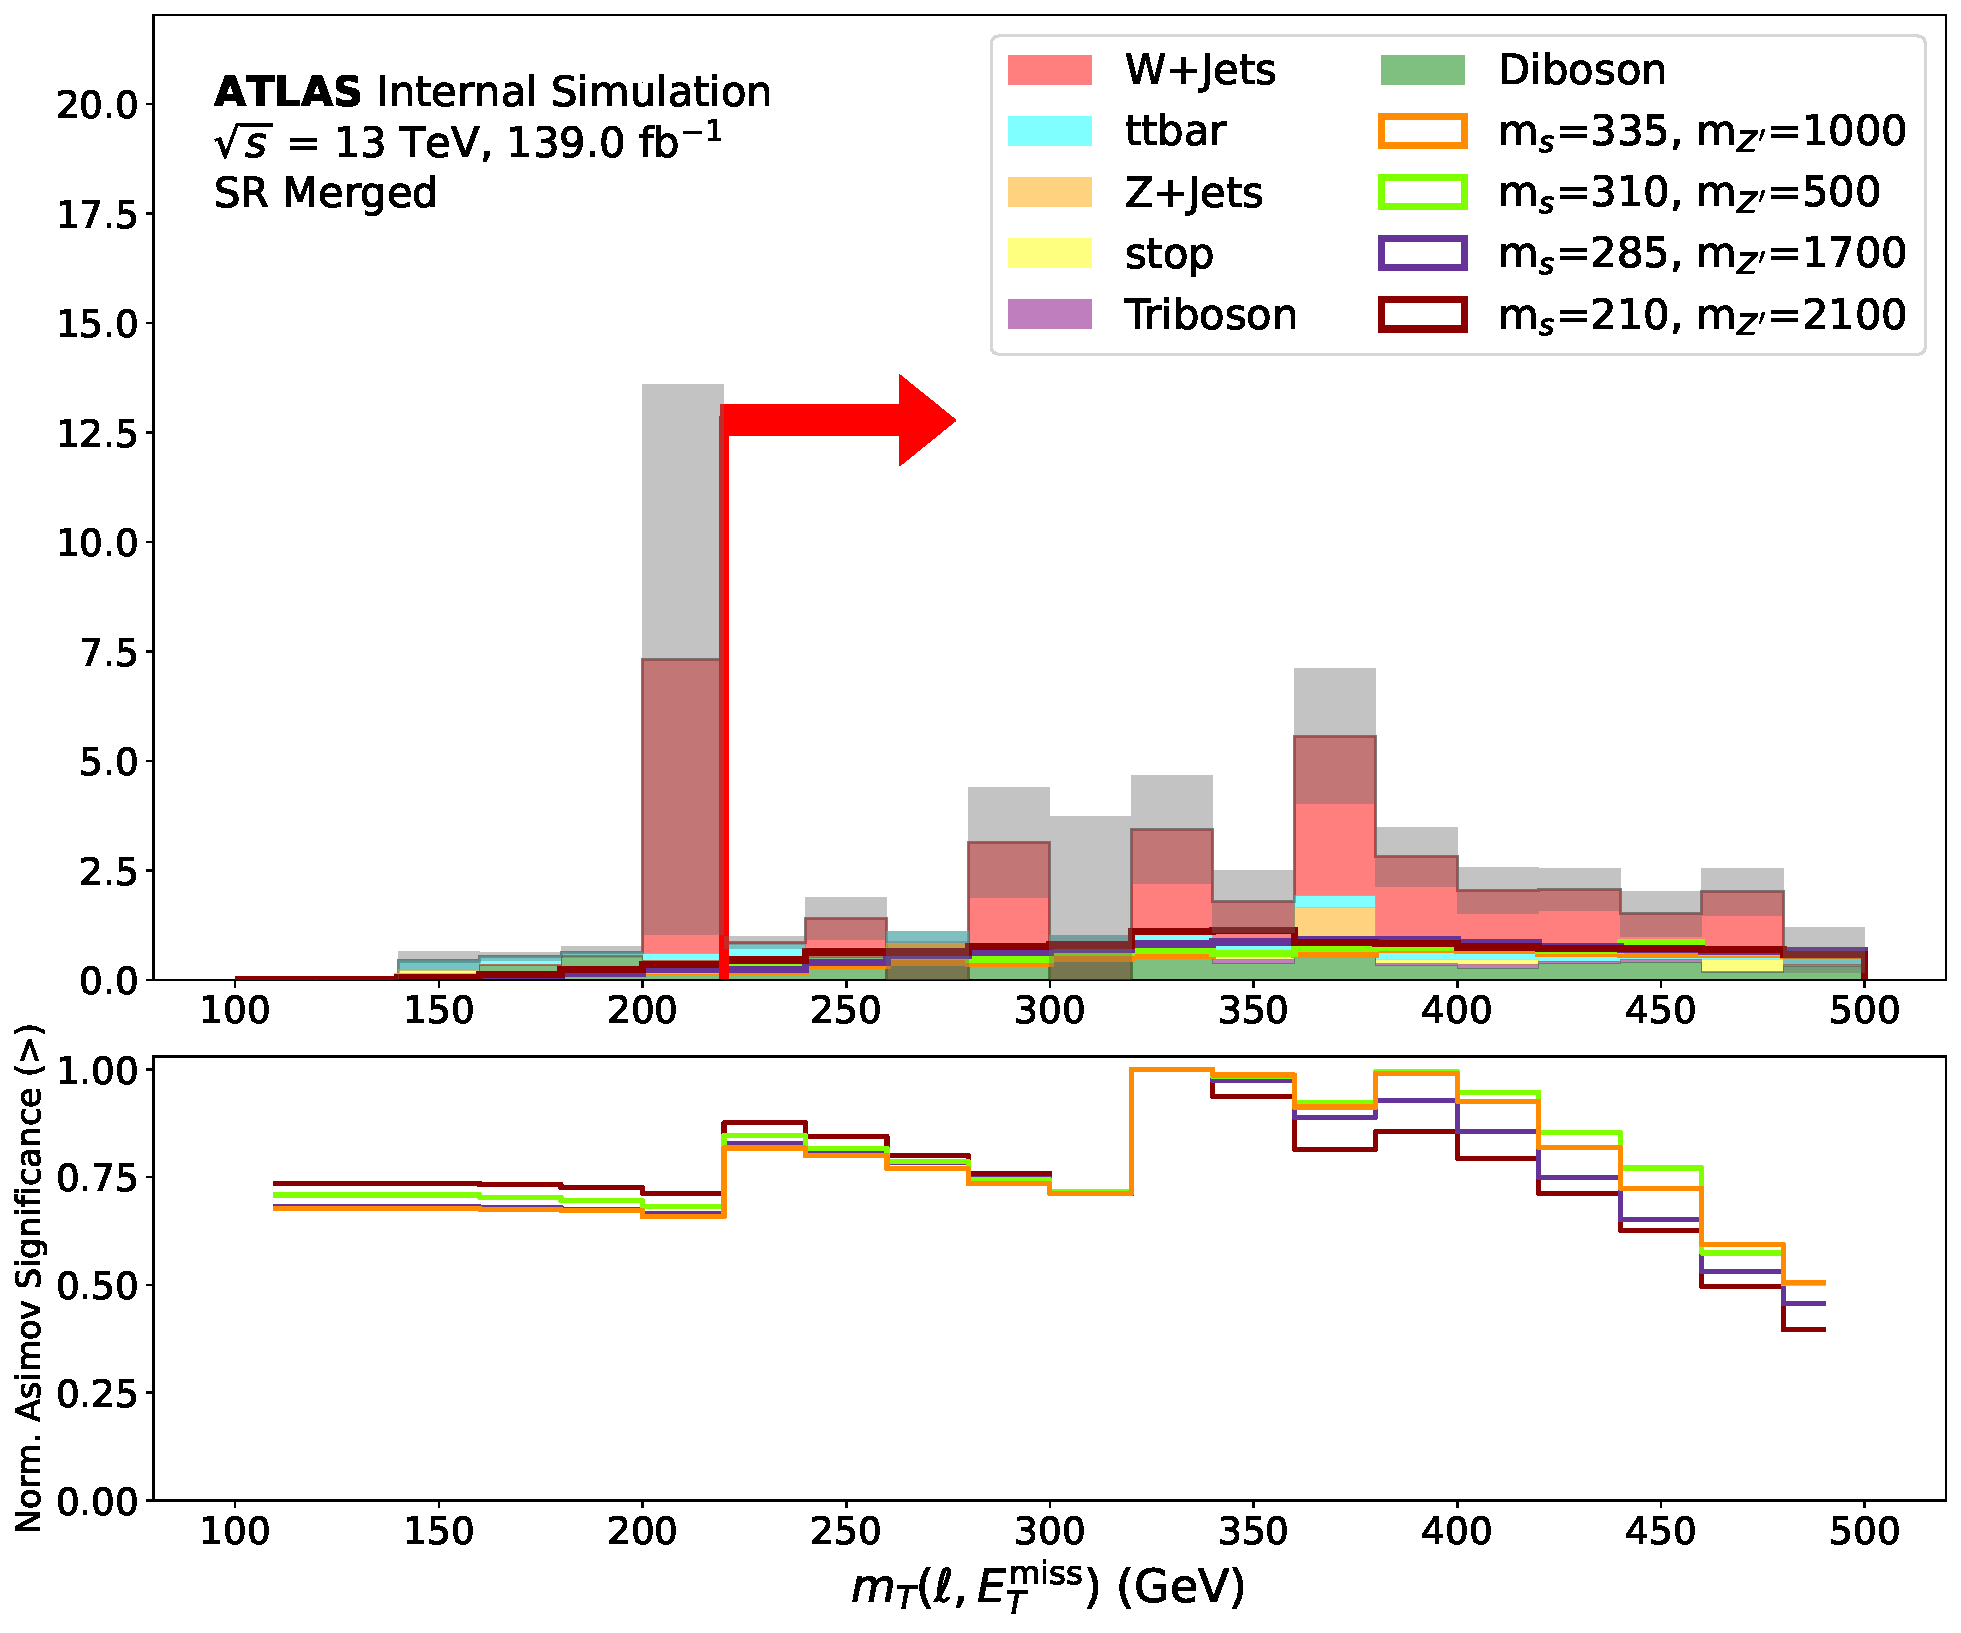
\includegraphics[width = 0.9\textwidth]{Figures/5/SR1L_Merged/mT_lep_met_normSig_N_1.pdf}
    \caption{\mtlepmet}
    \end{subfigure}
    \begin{subfigure}[t]{0.48\textwidth}
    \centering
     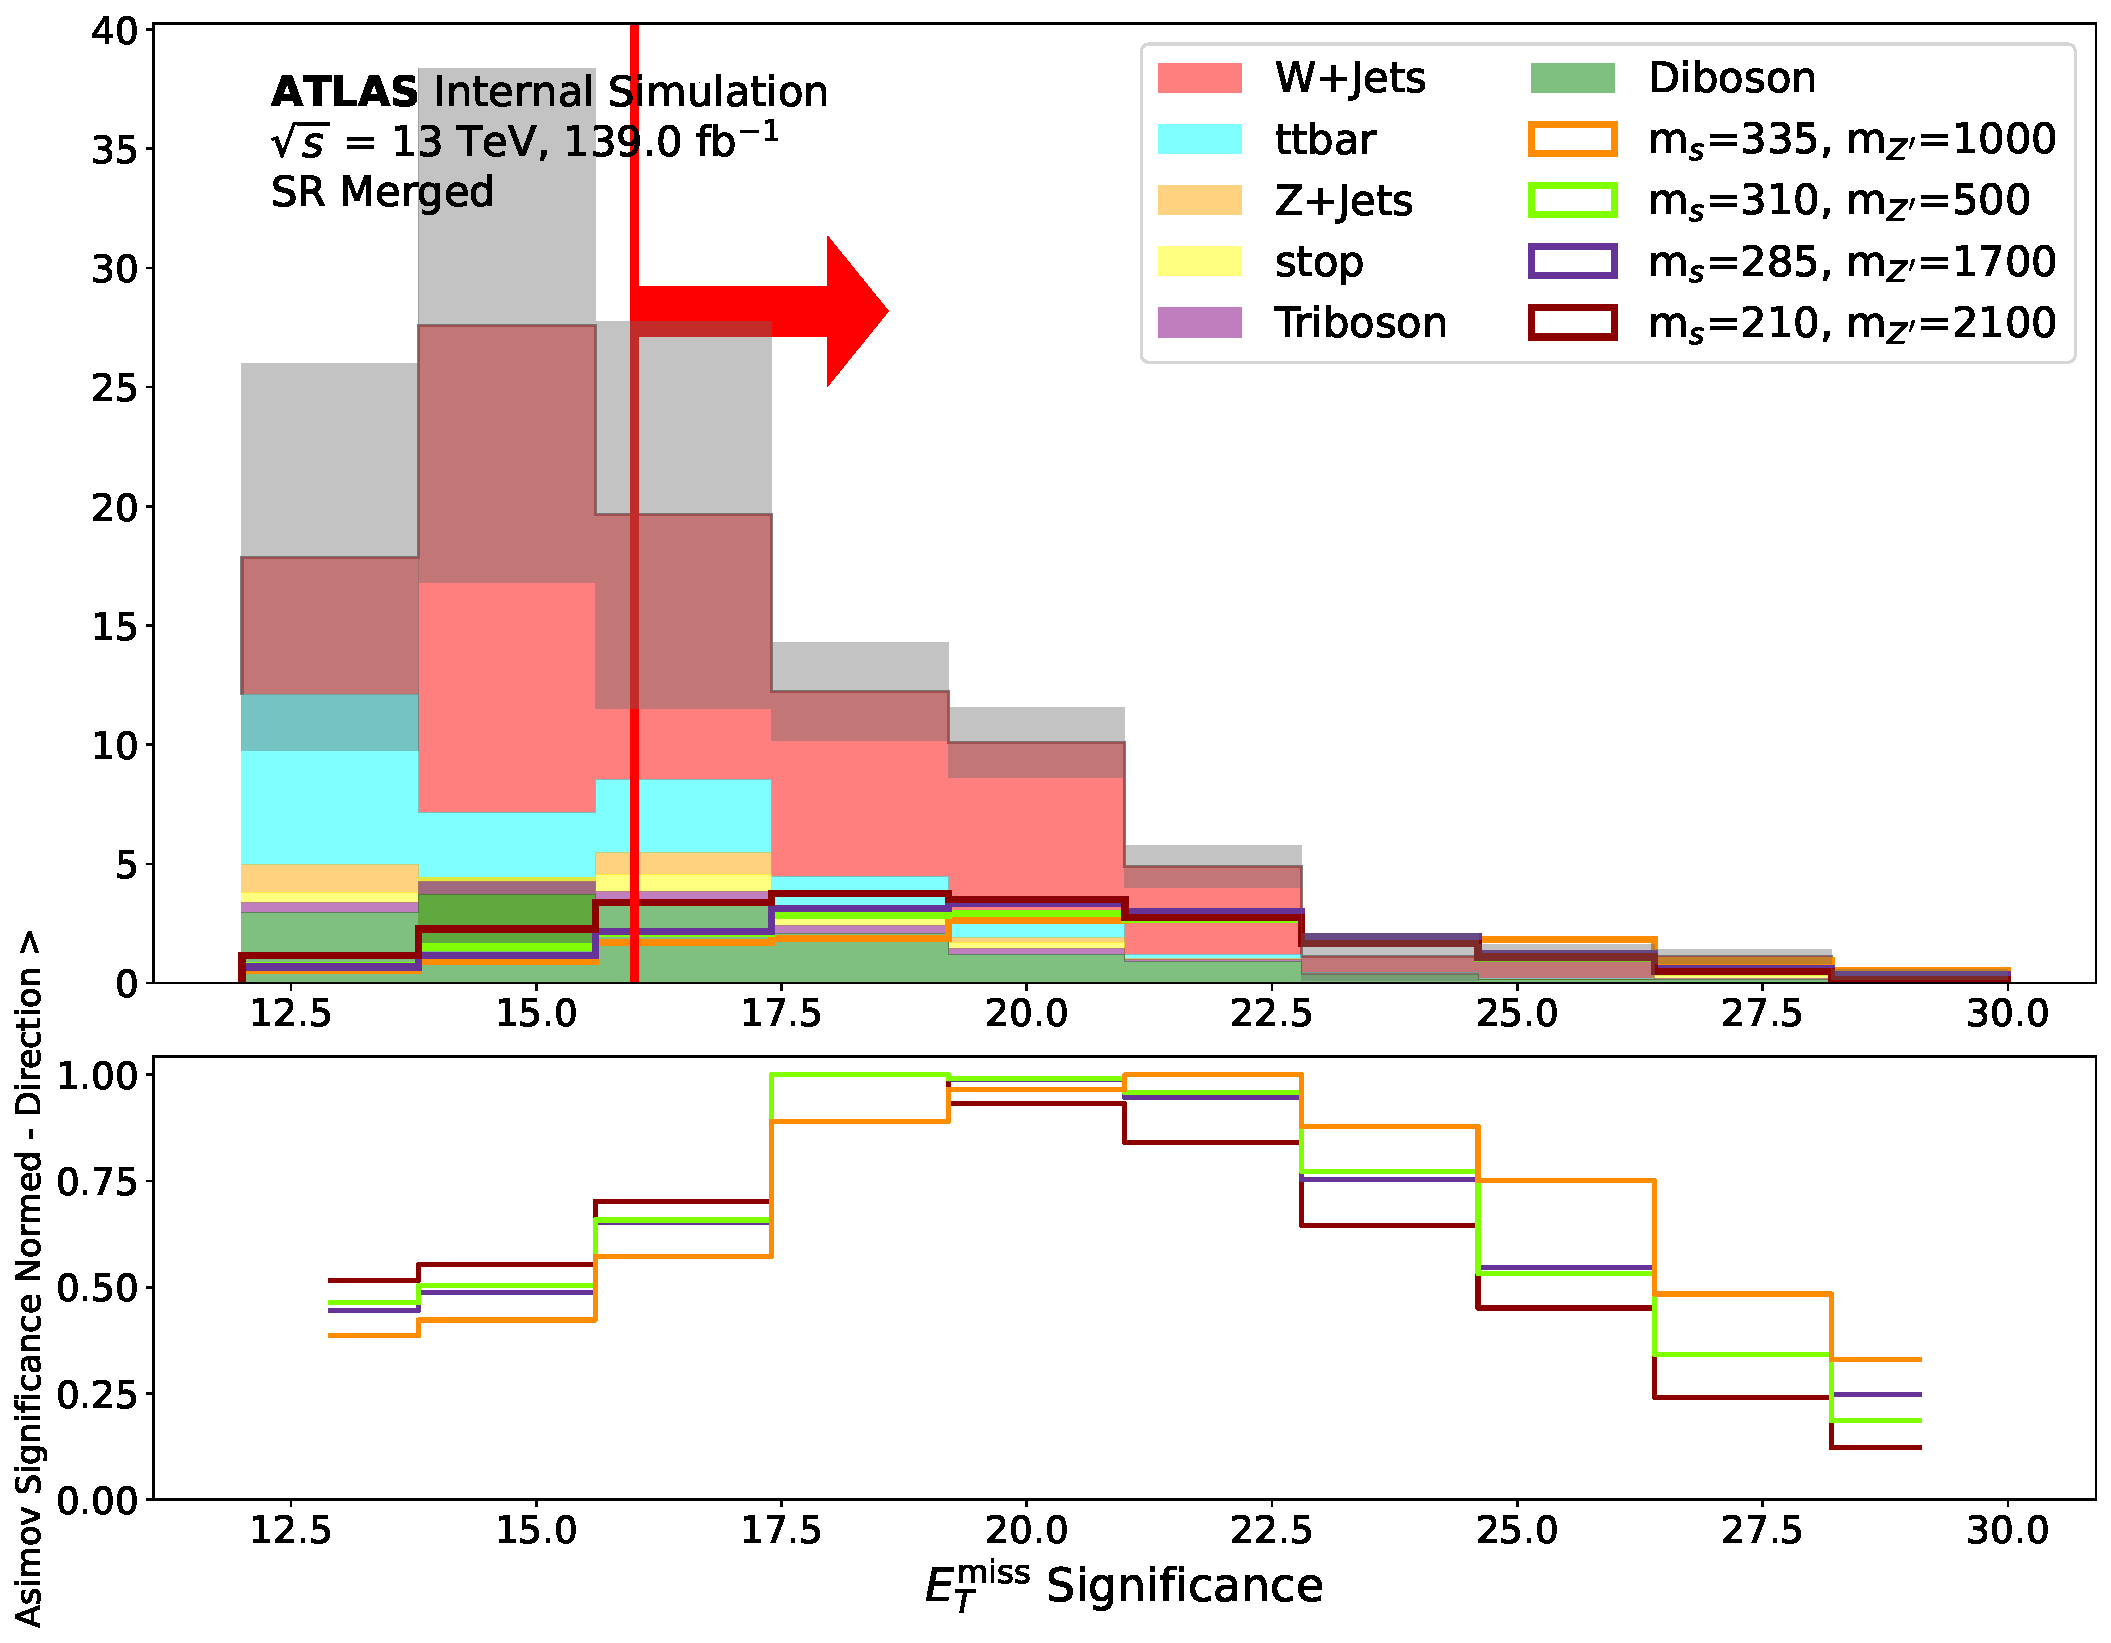
\includegraphics[width = 0.9\textwidth]{Figures/5/SR1L_Merged/MetTST_Significance_normSig_N_1.pdf}
    \caption{\metsig}
    \end{subfigure}
    \begin{subfigure}[t]{0.48\textwidth}
    \centering
     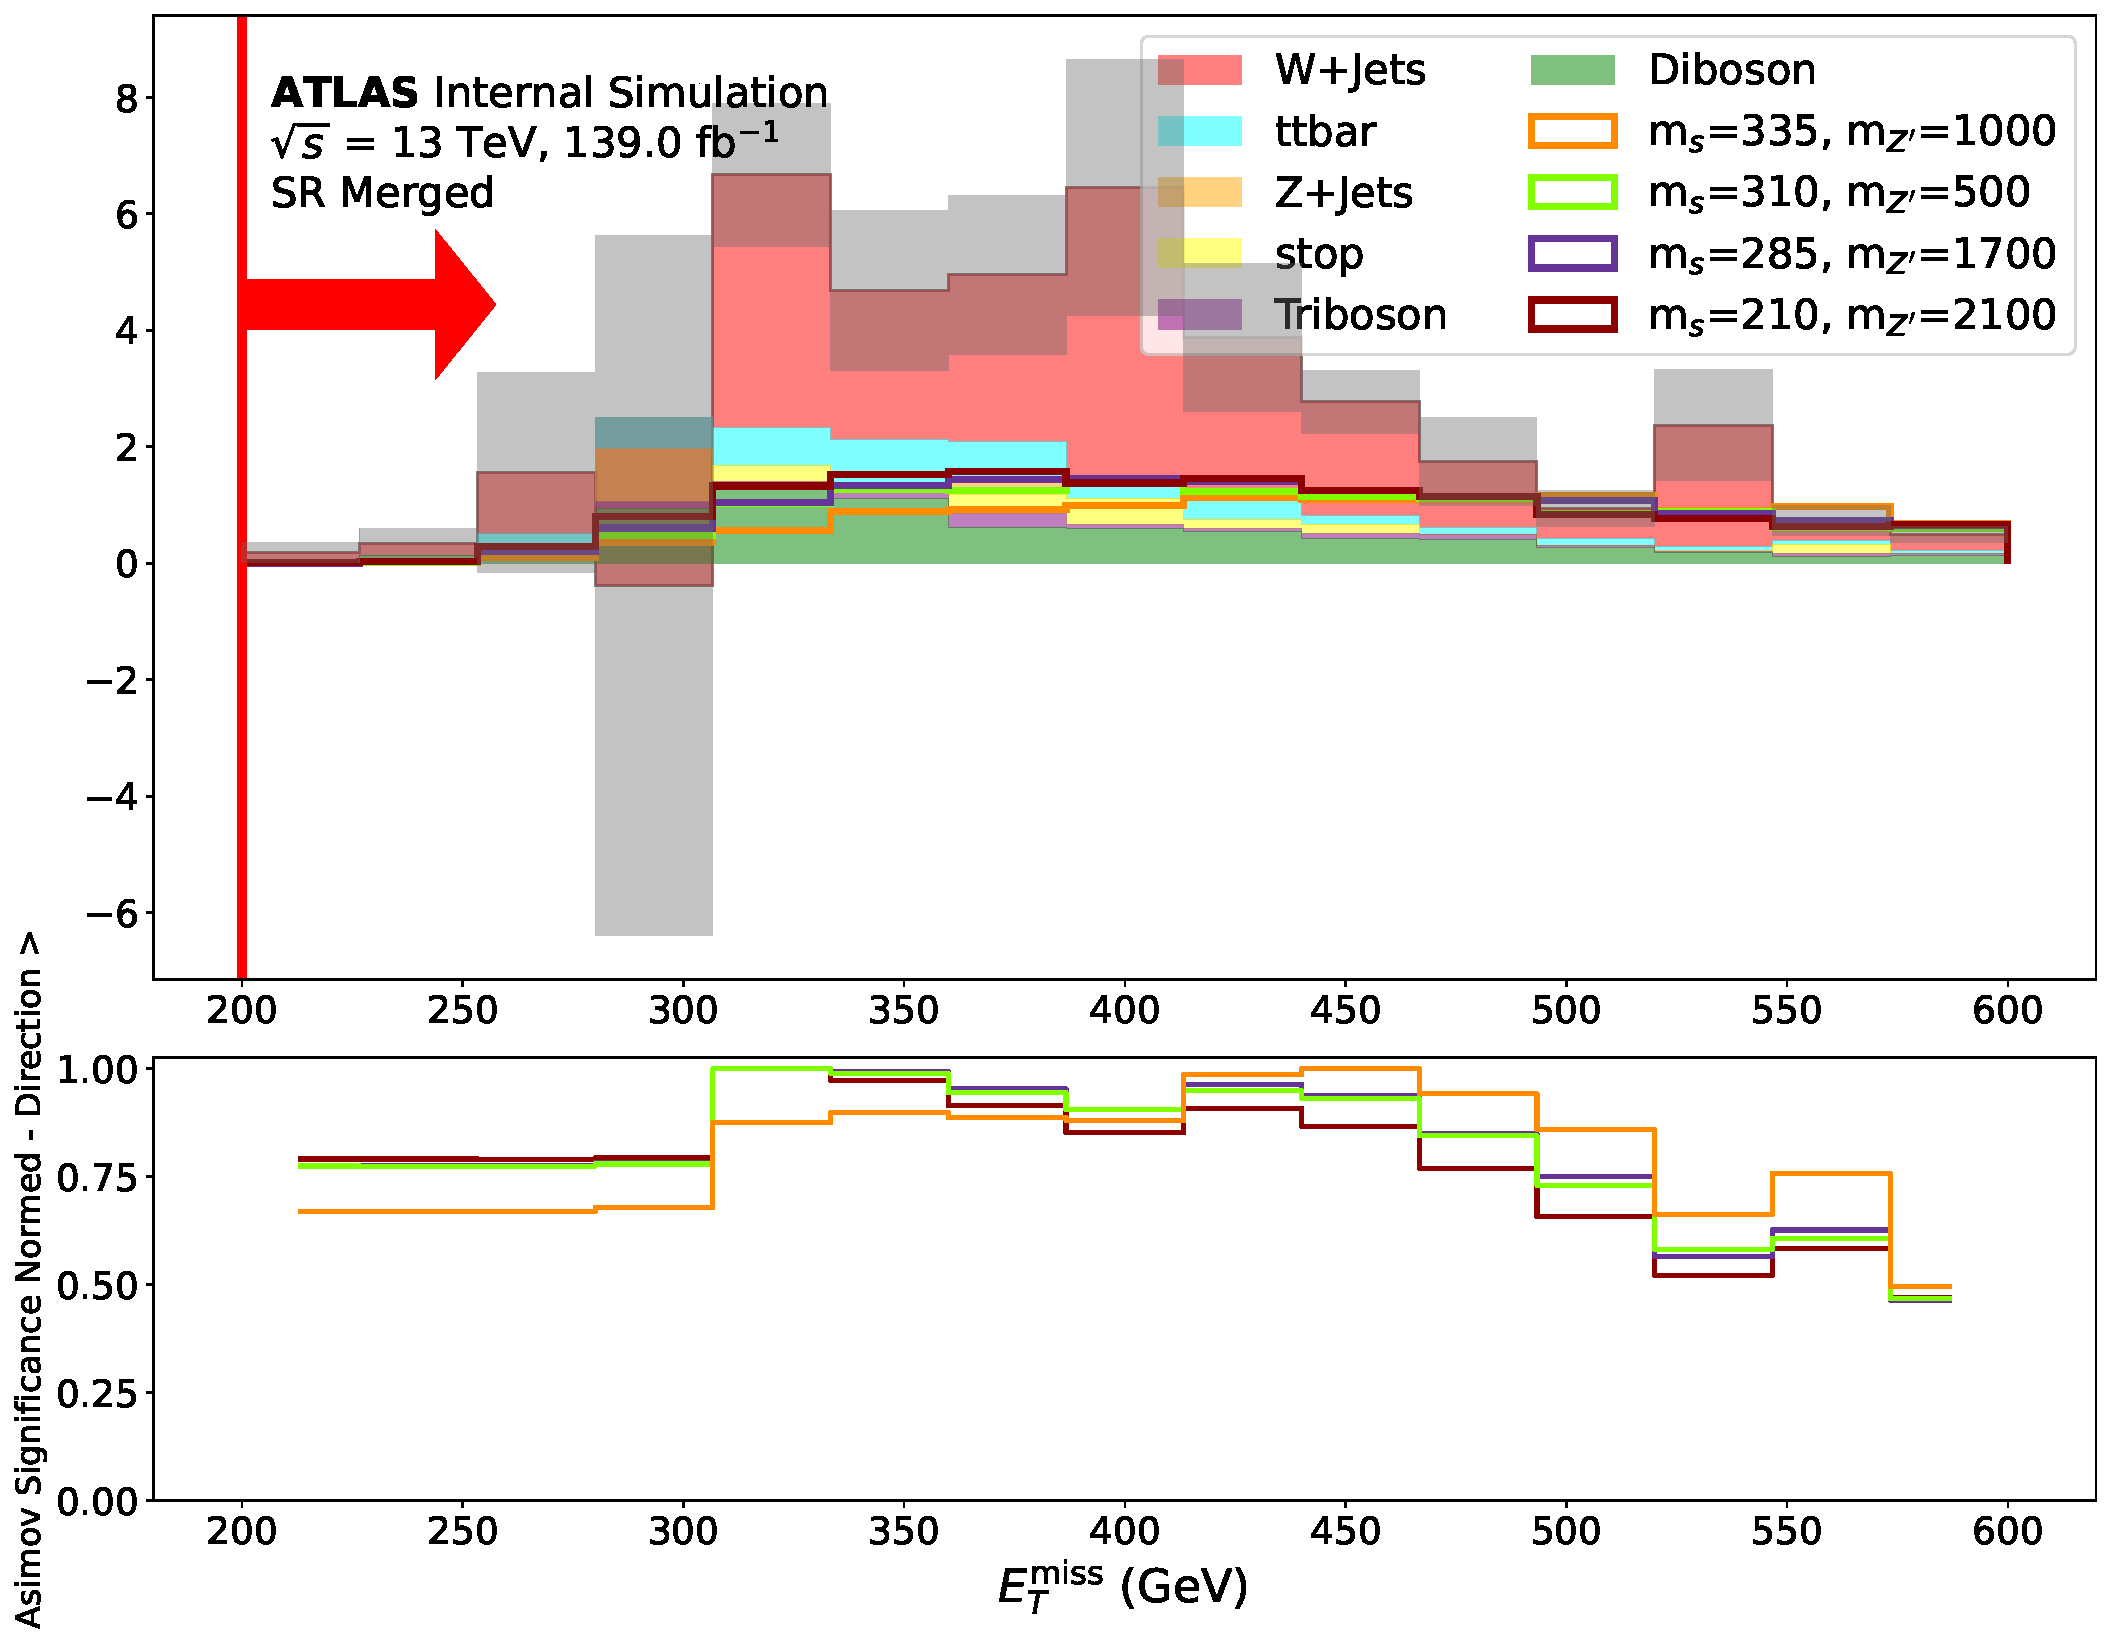
\includegraphics[width = 0.9\textwidth]{Figures/5/SR1L_Merged/MetTST_met_normSig_N_1.pdf}
    \caption{\met}
    \end{subfigure}
    \begin{subfigure}[t]{0.48\textwidth}
    \centering
     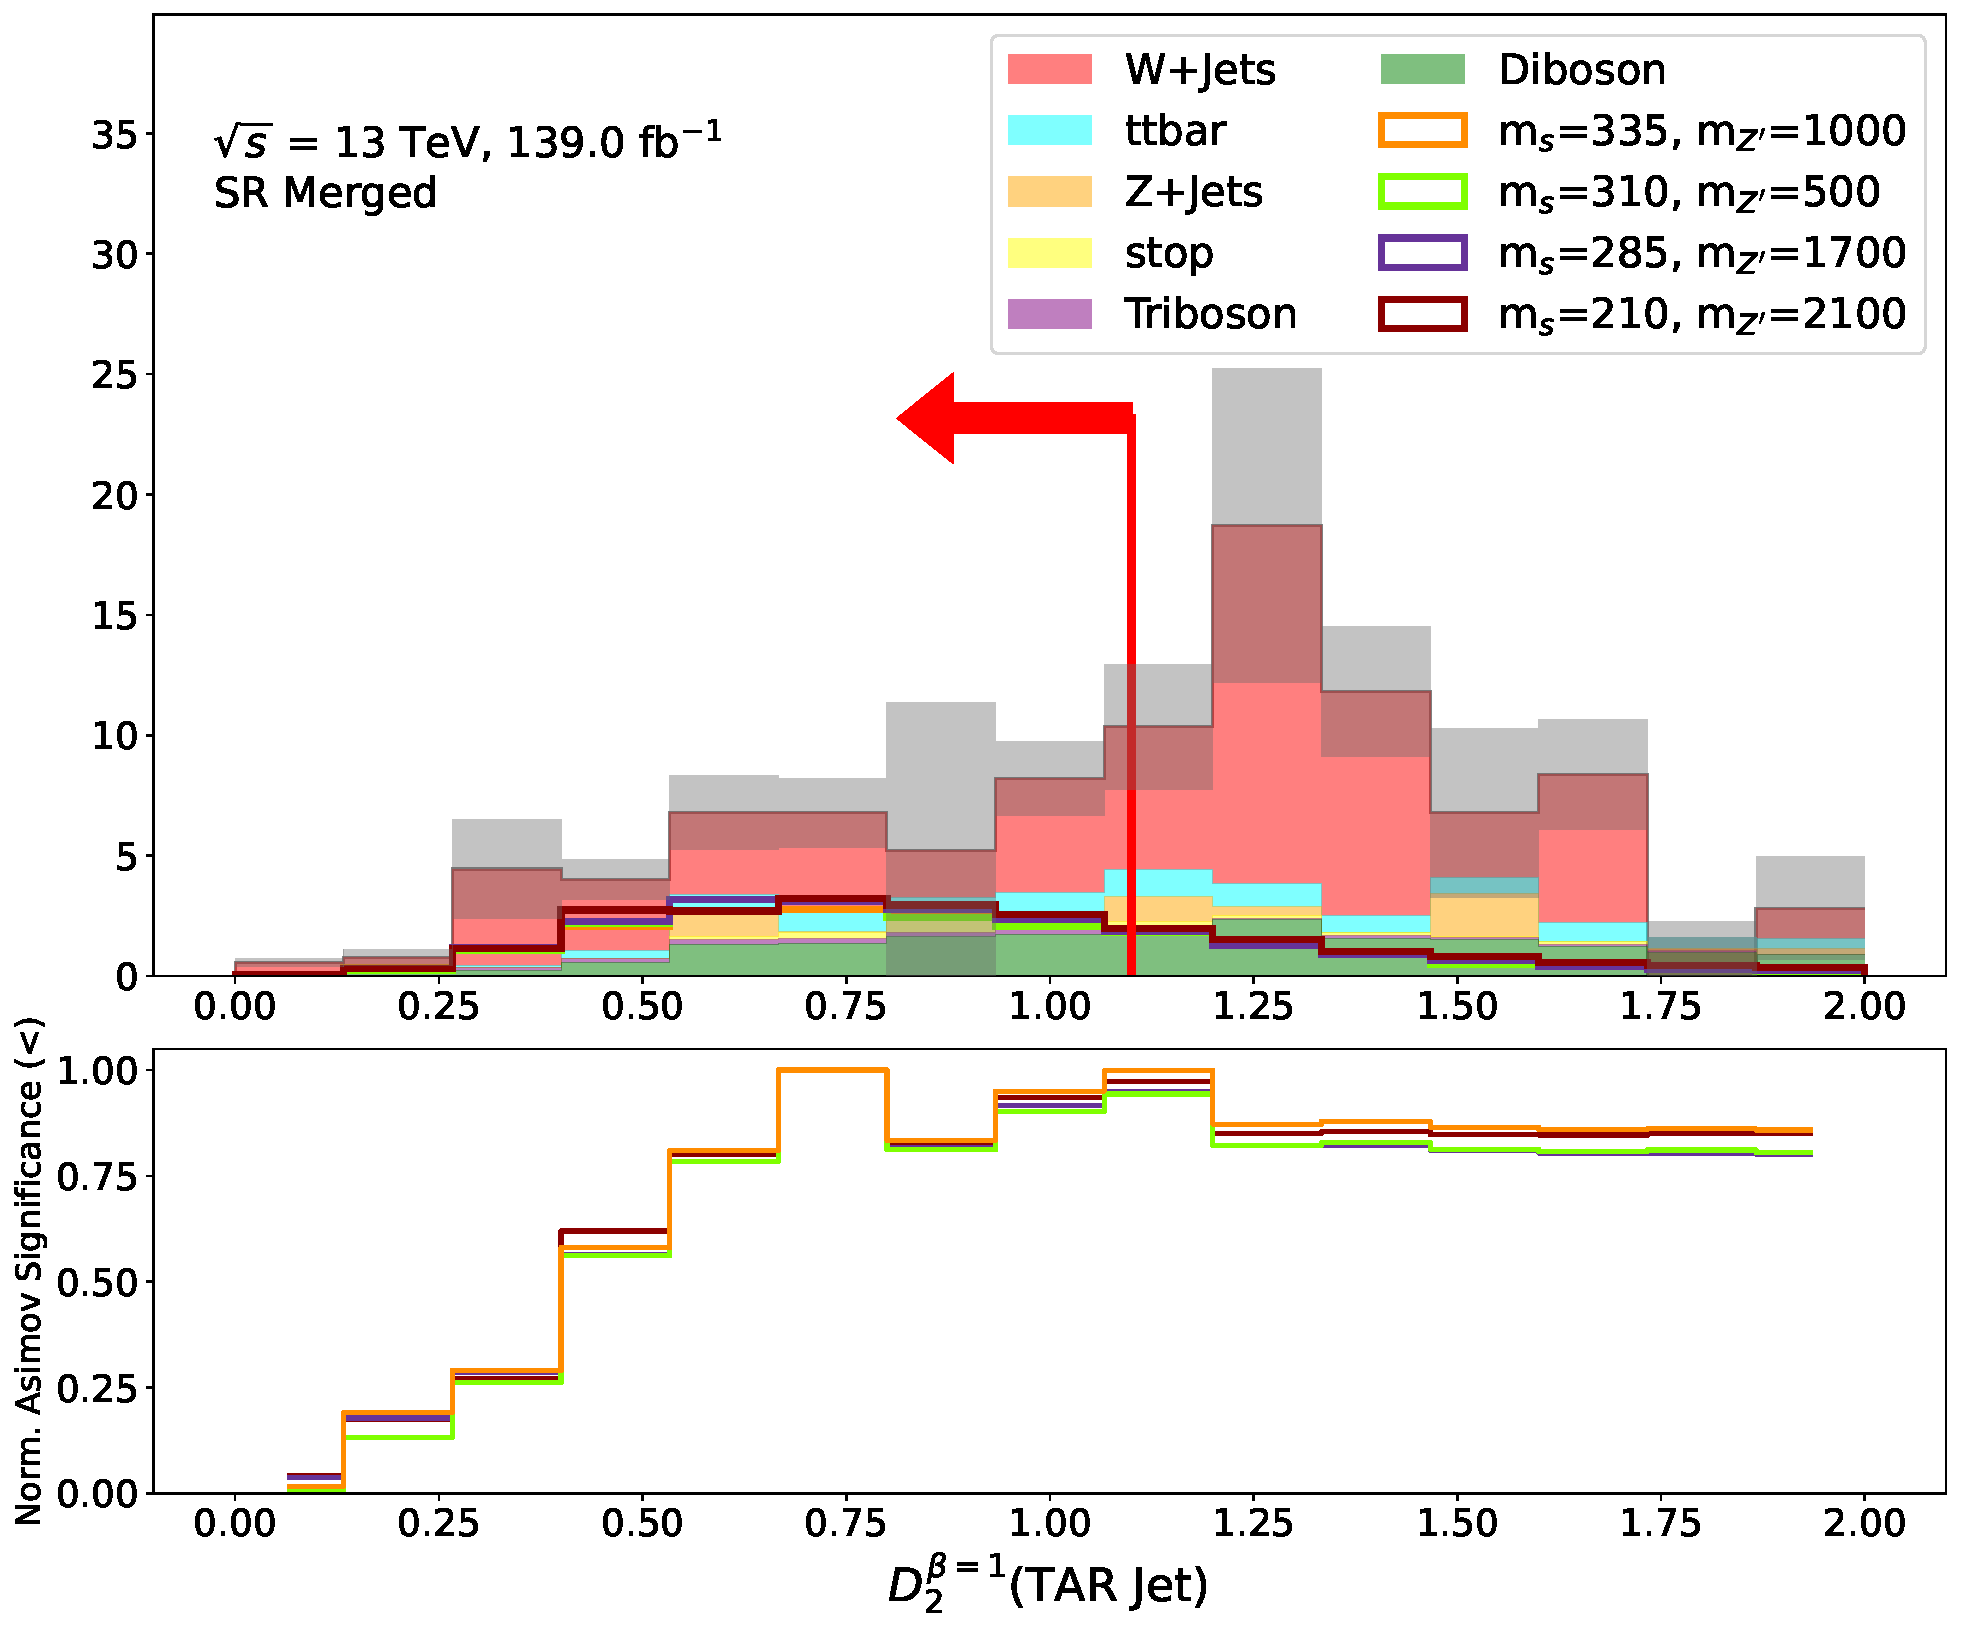
\includegraphics[width = 0.9\textwidth]{Figures/5/SR1L_Merged/TARJets10_TAR_D20_normSig_N_1.pdf}
    \caption{\DtwoTAR}
    \end{subfigure}
   \caption[N-1 Distributions for variables used in the merged signal region definition.]{N-1 Distributions for variables used in the merged signal region definition. Grey bands show statistical uncertainty on background estimate. The lower panel shows the cumulative Asimov significance normalized to unit peak, where the direction (\(>\) or \(<\)) specified in the y label indicates whether the significance is being summed from above (\(>\)) or from below (\(<\)). Red vertical line and arrow show placement and direction of selection on the given variable in this region.}
   \label{fig:Nminus1mergedSR_app}
\end{figure}
  
  
    \begin{figure}[htbp]
  \centering
    \begin{subfigure}[t]{0.48\textwidth}
    \centering
     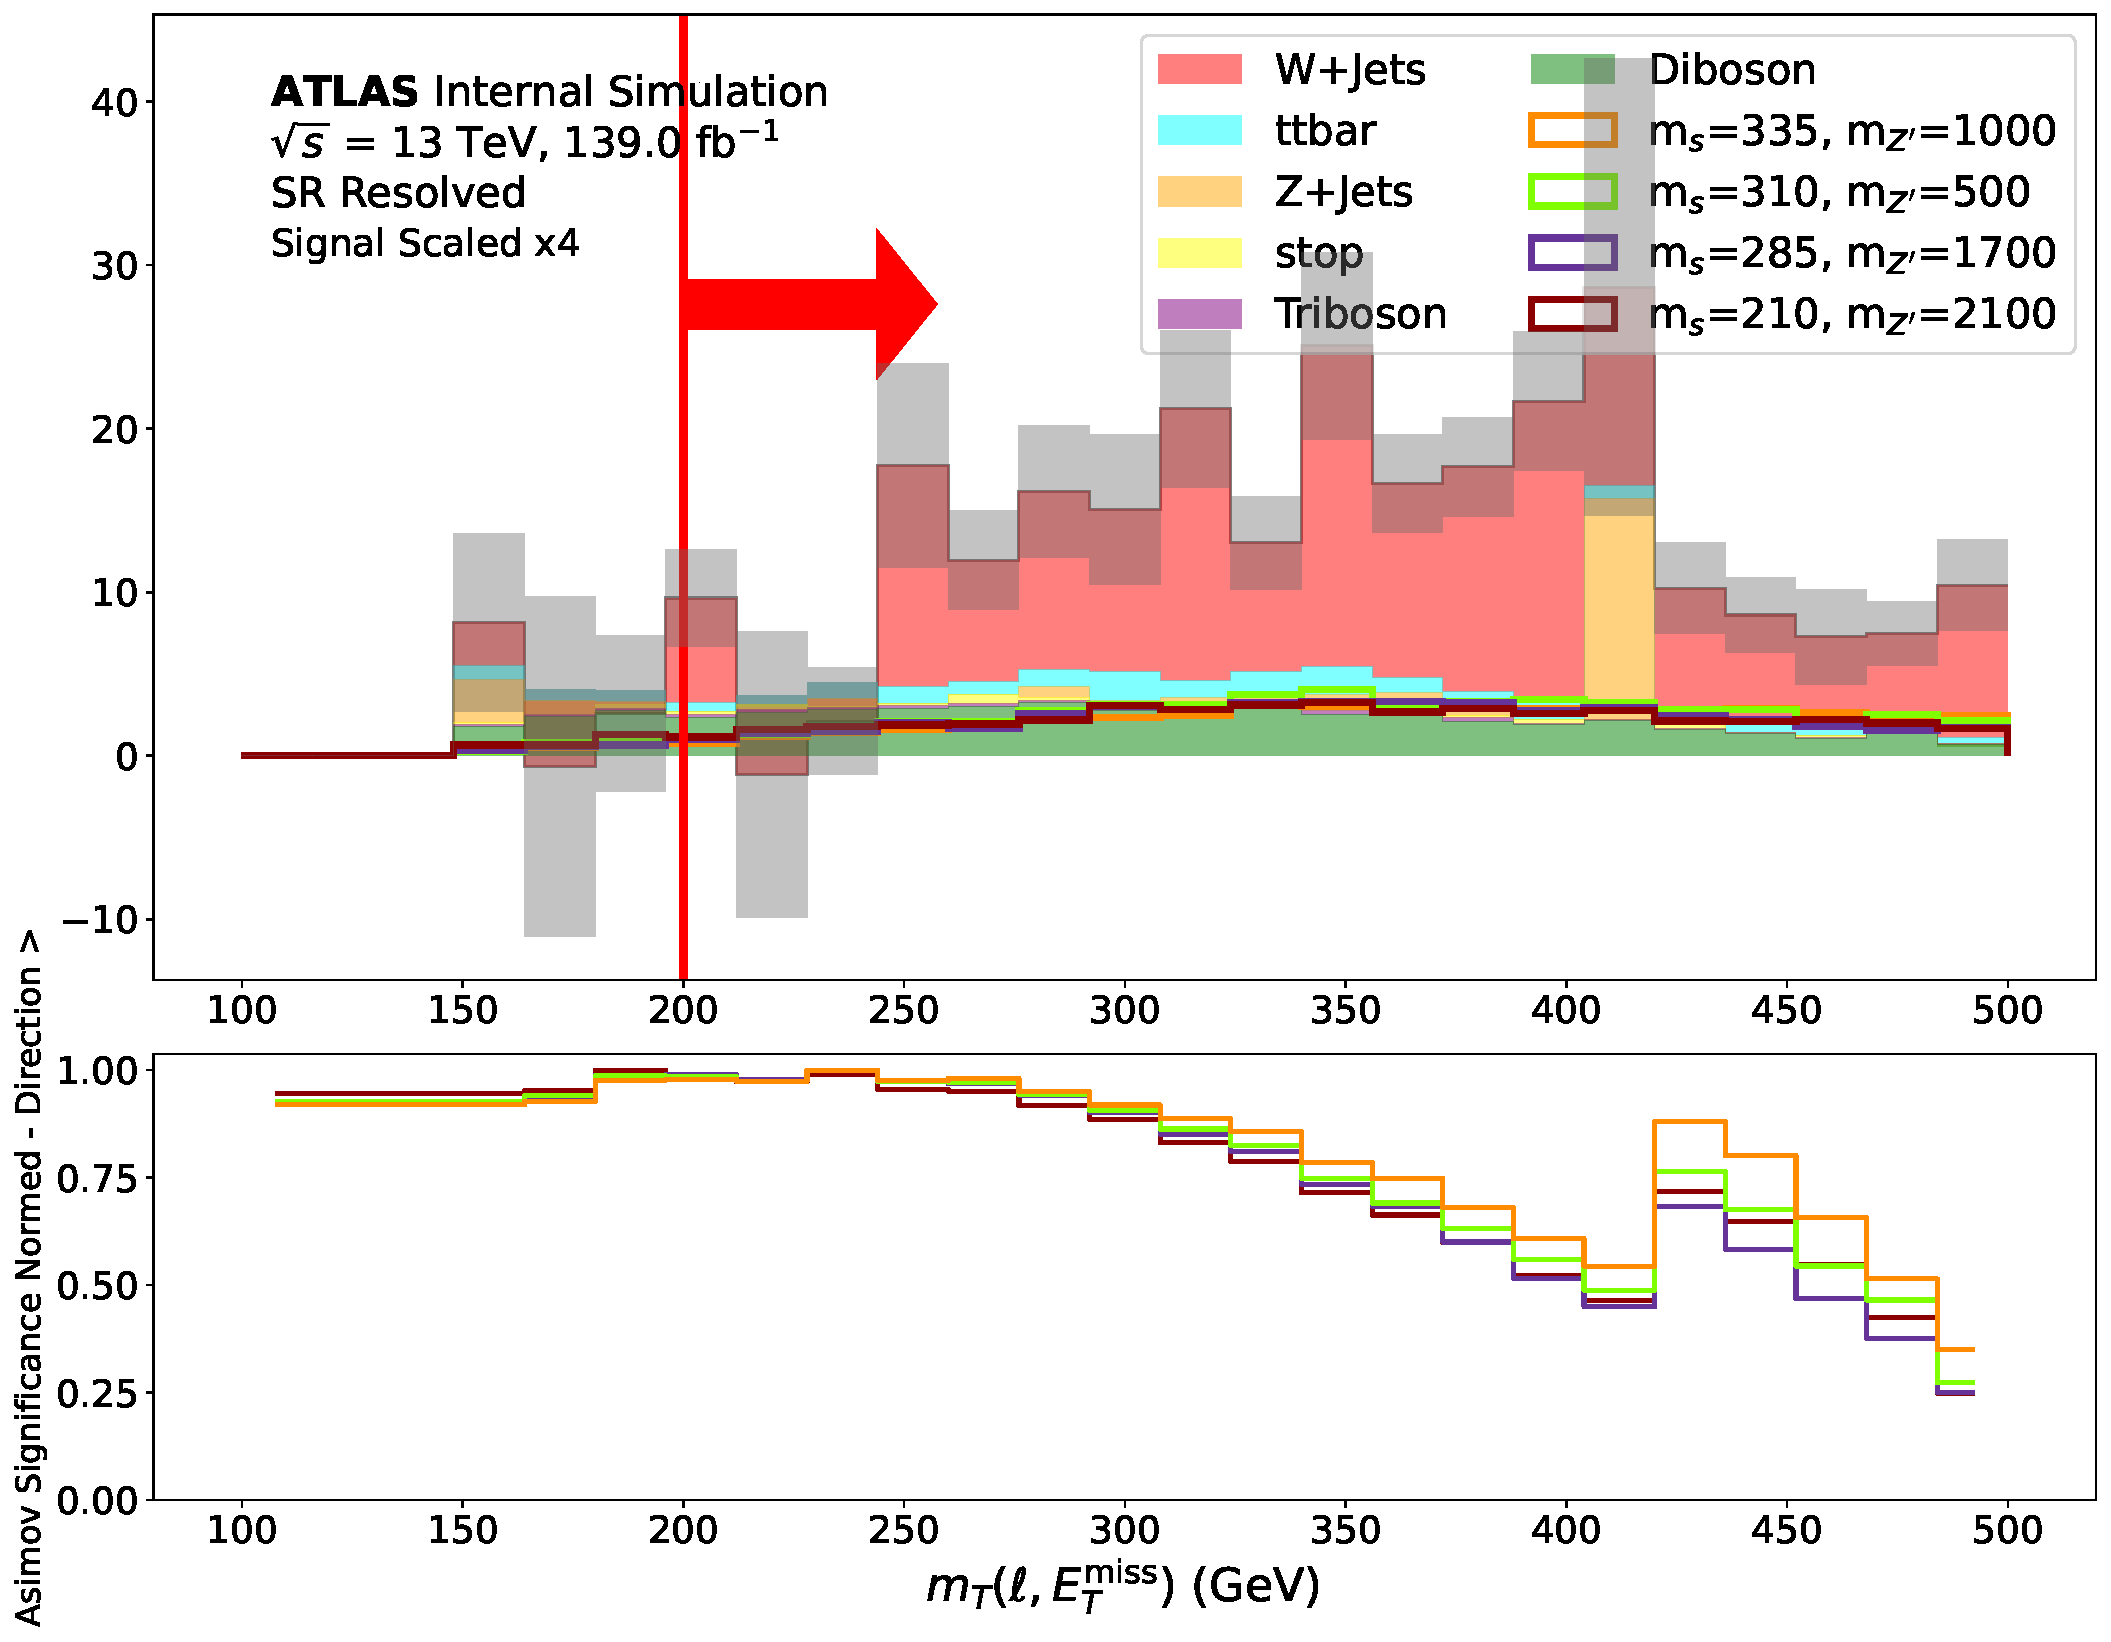
\includegraphics[width = 0.9\textwidth]{Figures/5/SR1L_Resolved/mT_lep_met_normSig_N_1.pdf}
    \caption{\mtlepmet}
    \end{subfigure}
    \begin{subfigure}[t]{0.48\textwidth}
    \centering
     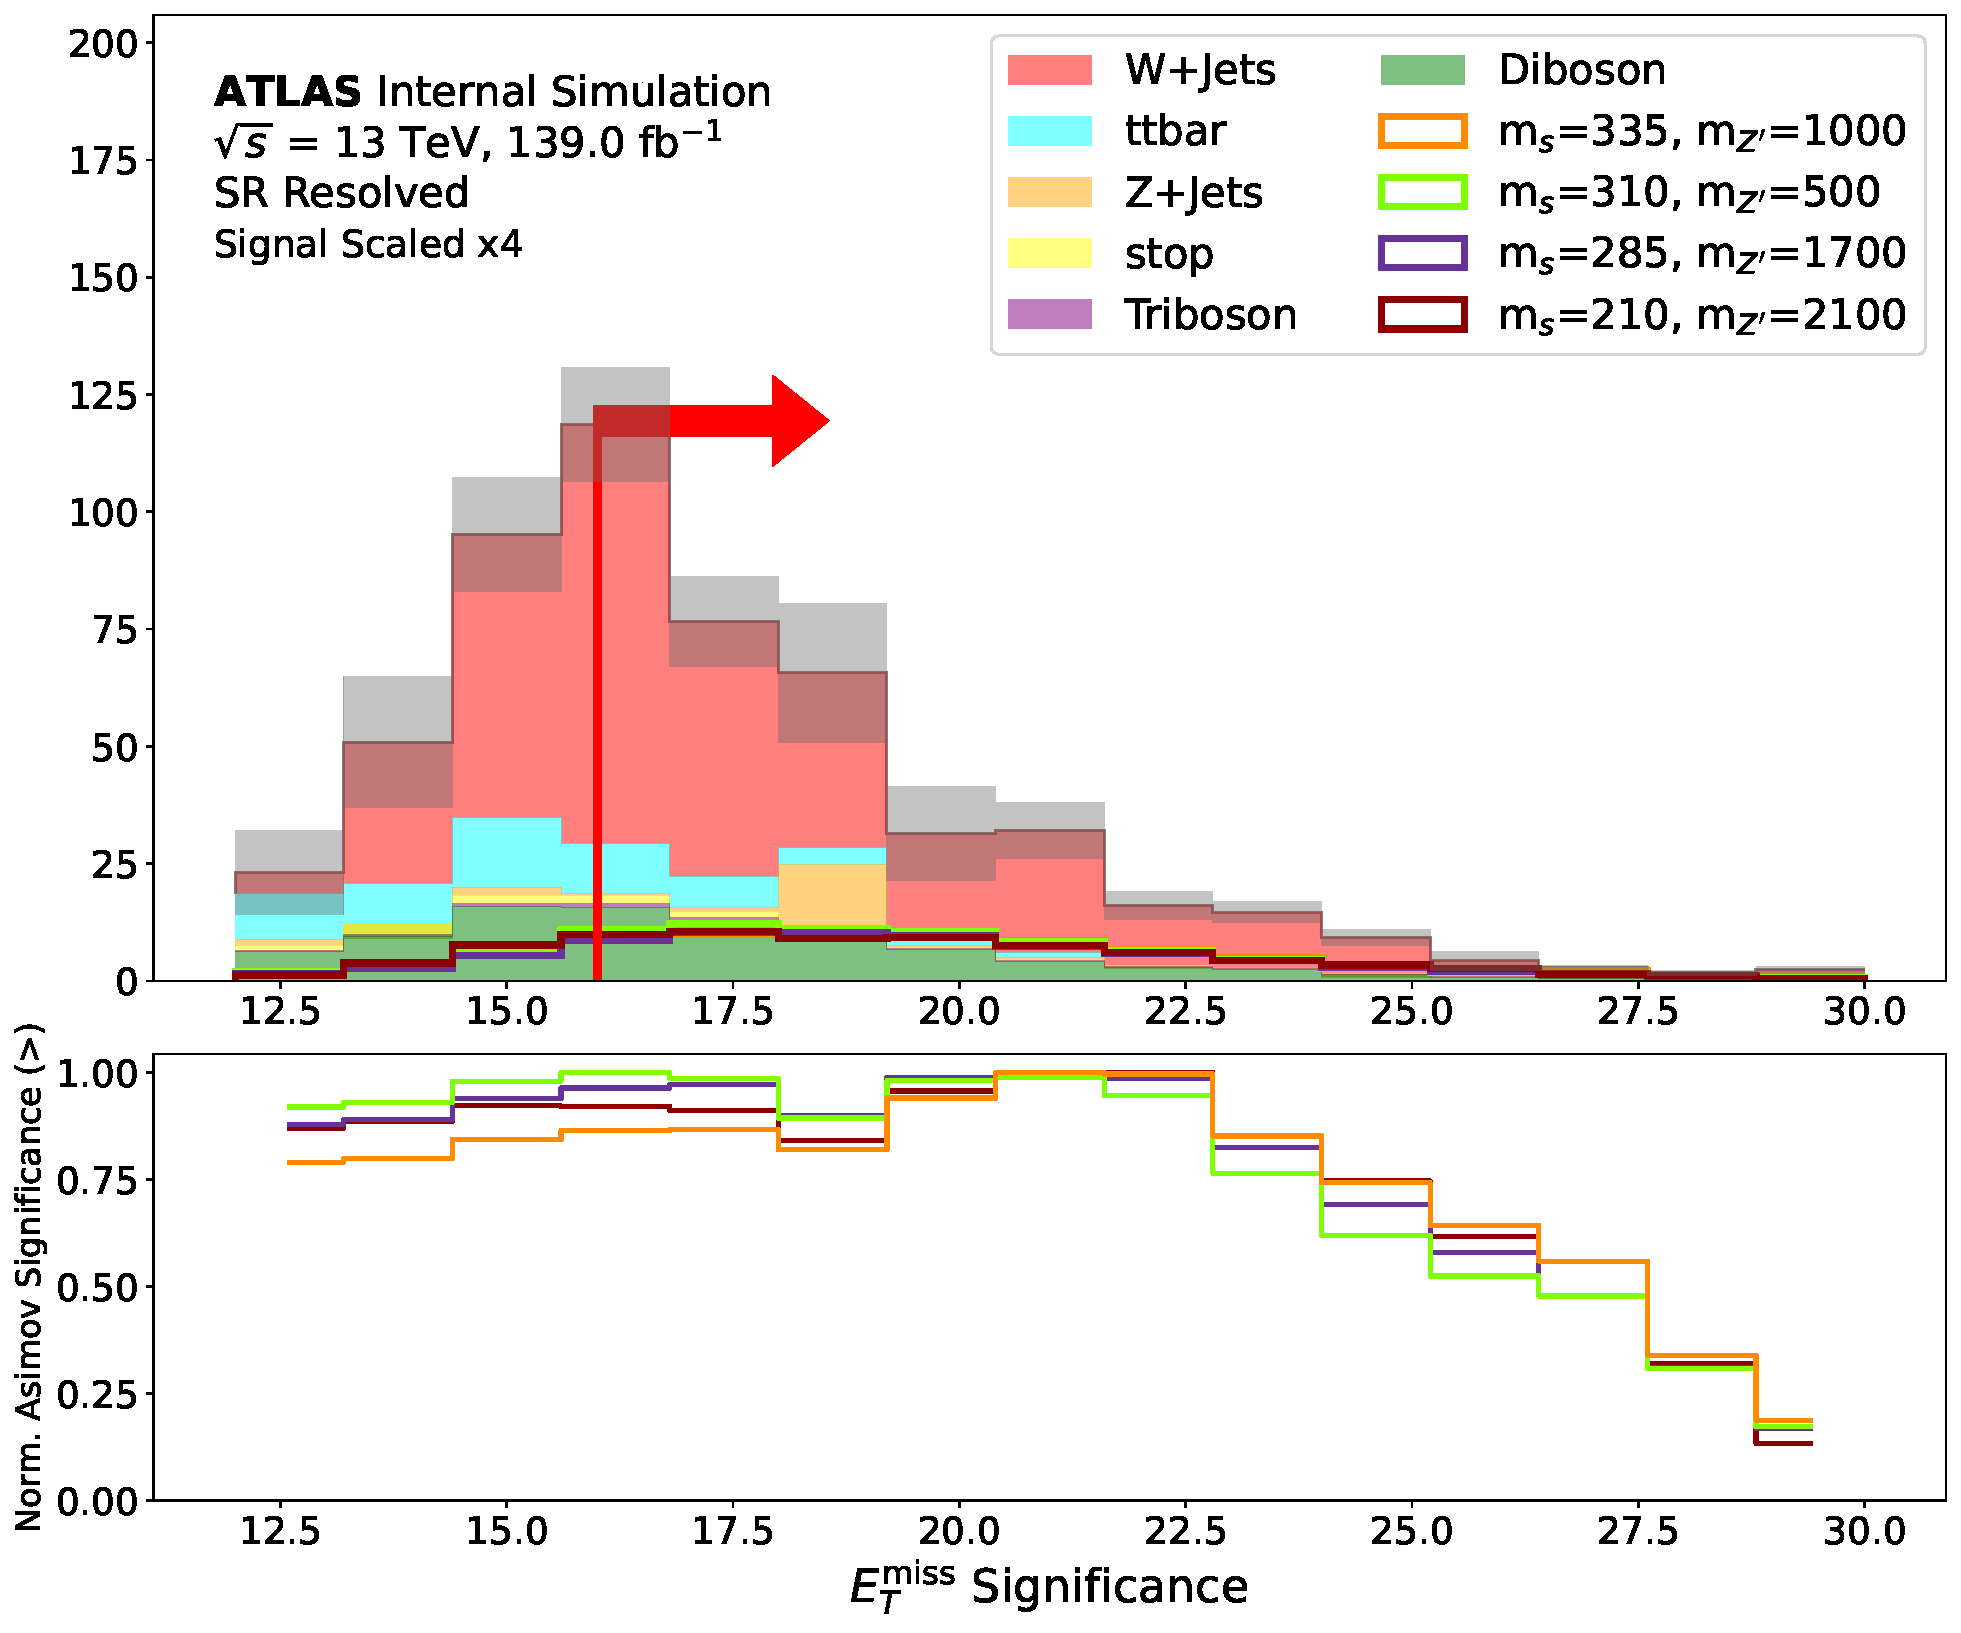
\includegraphics[width = 0.9\textwidth]{Figures/5/SR1L_Resolved/MetTST_Significance_normSig_N_1.pdf}
    \caption{\metsig}
    \end{subfigure}
    \begin{subfigure}[t]{0.48\textwidth}
    \centering
     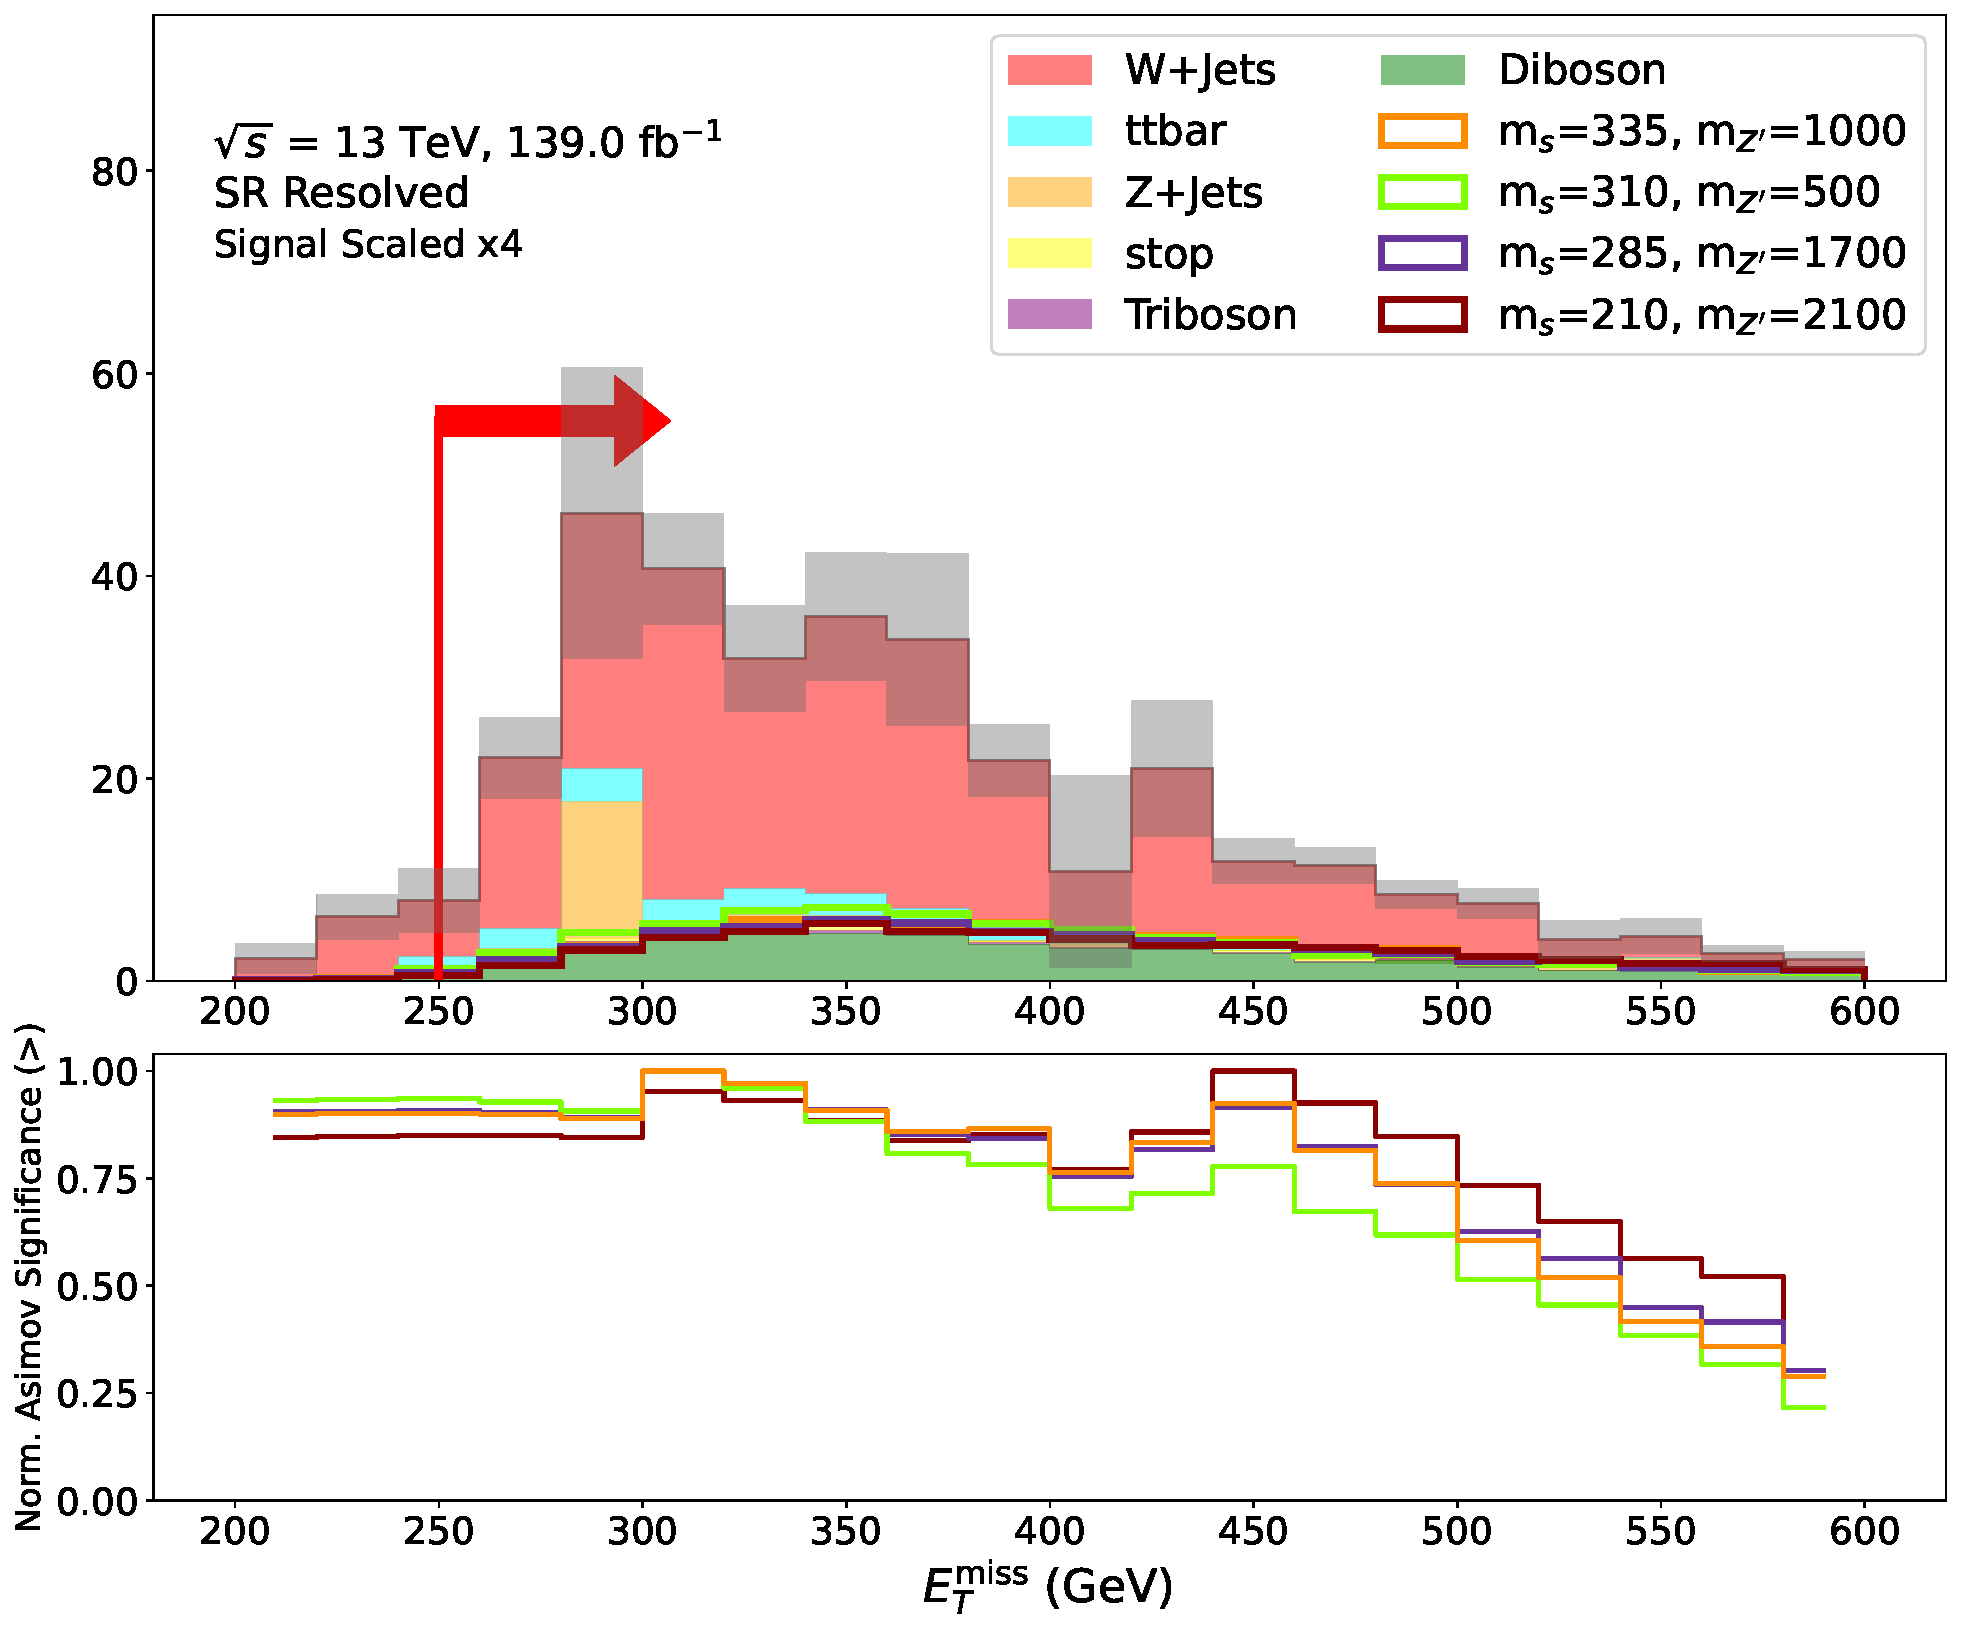
\includegraphics[width = 0.9\textwidth]{Figures/5/SR1L_Resolved/MetTST_met_normSig_N_1.pdf}
    \caption{\met}
    \end{subfigure}
    \begin{subfigure}[t]{0.48\textwidth}
    \centering
     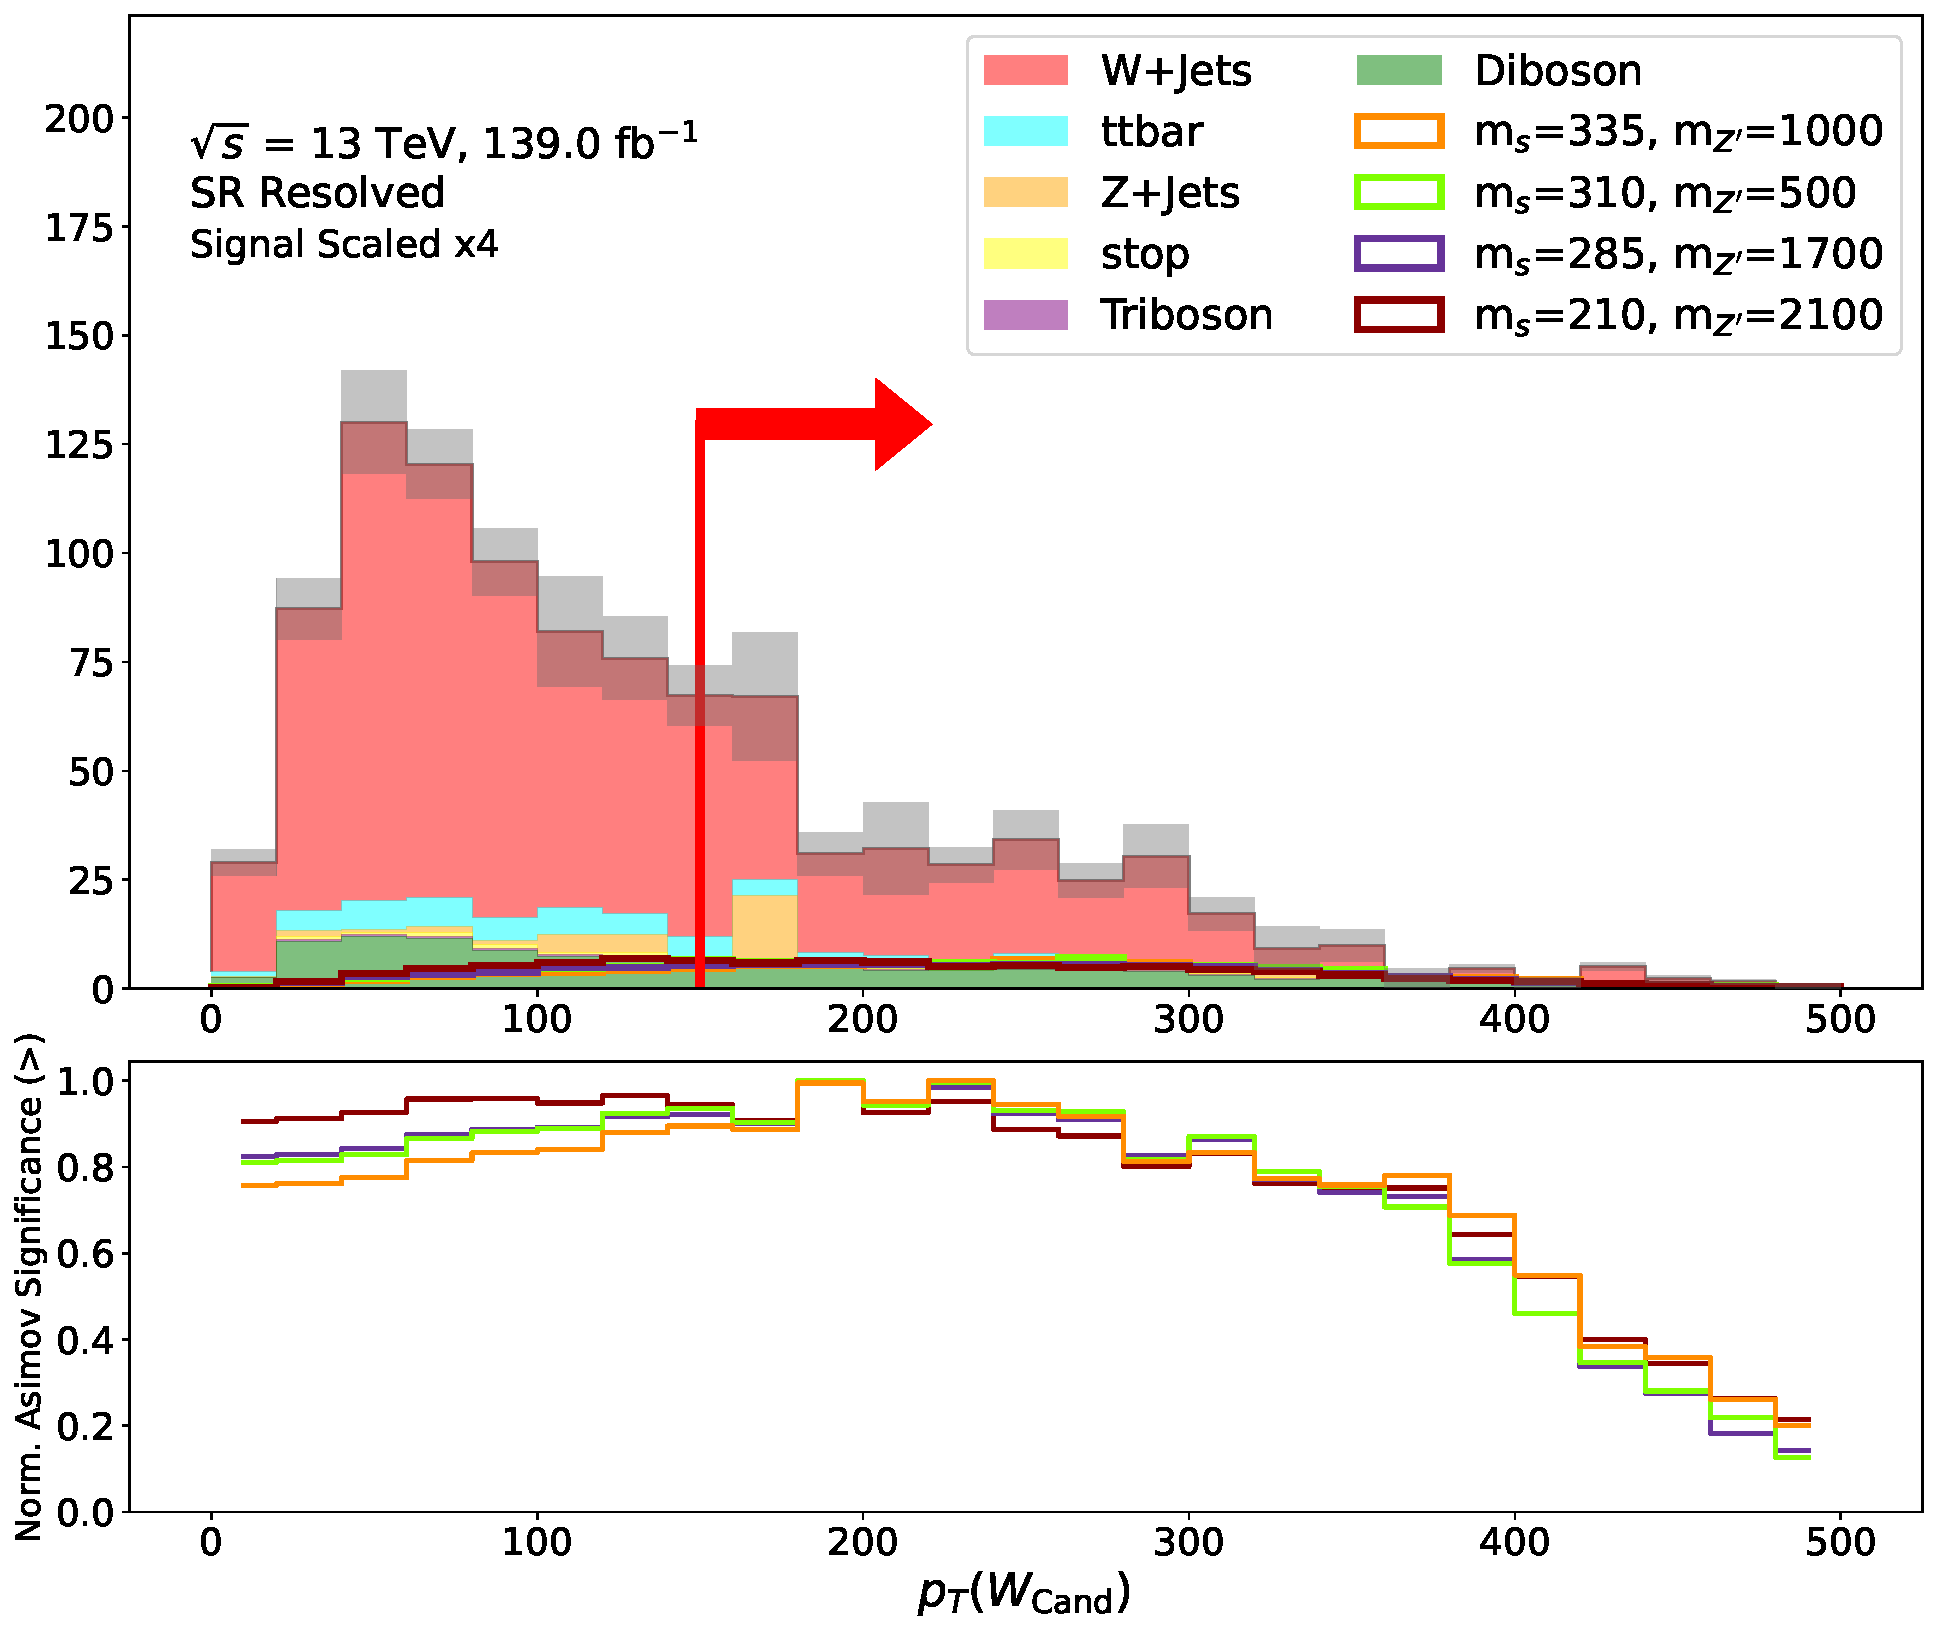
\includegraphics[width = 0.9\textwidth]{Figures/5/SR1L_Resolved/WCand_pt_normSig_N_1.pdf}
    \caption{\Wcandpt}
    \end{subfigure}
     \caption[N-1 Distributions for variables used in the resolved signal region definition.]{N-1 Distributions for variables used in the resolved signal region definition. Grey bands show statistical uncertainty on the background estimate. The lower panel shows the cumulative Asimov significance normalized to unit peak, where the direction (\(>\) or \(<\)) specified in the y label indicates whether the significance is being summed from above (\(>\)) or from below (\(<\)). Red vertical line and arrow show placement and direction of selection on the given variable in this region.}
     \label{fig:Nminus1resolvedSR_app}
\end{figure}